\section{Durchführung}
\label{sec:Durchführung}
Für den Versuch stehen ein Ultraschallechoskop, Ultraschallsonden die 1 oder 2 MHz emittieren, einen Rechner zur Datenaufnahme und -analyse, ein Acrylblock und ein Brustimitat zur Verfügung.

\subsection{Untersuchung eines Acrylblocks mit dem A-Scan}
Zu erst ist der Acrylblock mit einer Schieblehre auszumessen, sowie der Durchmesser der Fehlstellen und der Abstand der Anfangspunkte der Fehlstellen in Relation zur unteren und oberen Seite des Acrylblocks.
Dann wird das Kontaktmittel bidestilliertes Wasser auf den Acrylblock gesetzt und mit der 2MHz Sonde und dem Impuls-Echo-Verfahren die Schallaufzeiten auf beiden Seiten gemessen, um die Lage der Bohrungen innerhalb des Acrylblocks zu messen.  
\begin{figure}[H]
  \centering
  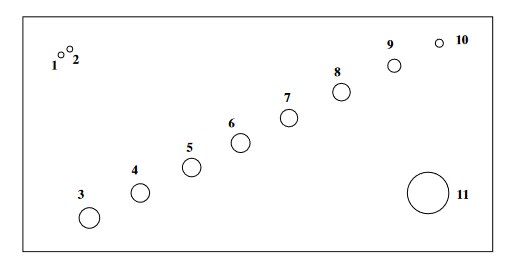
\includegraphics[width=9cm]{content/block}
  \caption{Skizze des verwendeten Acrylblocks. \cite{1}}
\end{figure}

\subsection{Untersuchung des Auflösungsvermögens}
Zur Untersuchung des Auflösungsvermögens wird die 2 MHz Sonde an den nebeneinanderstehenden kleinen Fehlstellen gescanned und das Auflösungsvermögen beurteilt.

\subsection{Untersuchung eines Acrylblocks mit dem B-Scan}
Die 2 MHz Sonde wird über beide Seiten des mit Kontakmittel versehenen Acrylblocks geführt, um die Fehlstellen zu messen. 

\subsection{Untersuchung eines Brustmodells mit einem B-Scan}
Das Brustmodell wird mit dem Kontaktmittel versehen. Dann werden mit dem A-Scan die eingesetzten Objekte abgetastet und über den B-Scan die Tiefe und Größe der Tumormodelle innerhalb des Brustmodells bestimmt.
